% ch07_matplotlib.tex — Matplotlib : Visualisation Scientifique
\chapter{Matplotlib --- Visualisation Scientifique}
\label{ch:matplotlib}

\begin{intuition}
<<~Une image vaut mille mots~>>, et en science, un graphique vaut mille tableaux
de donn\'ees. Matplotlib\index{Matplotlib} est la biblioth\`eque de r\'ef\'erence en Python
pour cr\'eer des figures de qualit\'e publication. Pensez-y comme le
<<~papier millim\'etr\'e num\'erique~>> du scientifique moderne.
\end{intuition}

% ============================================================
\section{Premier graphique~: \py{plt.plot()}}
\index{plt.plot}

\begin{codeblock}[title=\textbf{Python}]
\begin{minted}{python}
import numpy as np
import matplotlib.pyplot as plt

x = np.linspace(0, 2 * np.pi, 200)
y_sin = np.sin(x)
y_cos = np.cos(x)

plt.plot(x, y_sin, label="sin(x)")
plt.plot(x, y_cos, label="cos(x)", linestyle="--")
plt.xlabel("x (radians)")
plt.ylabel("y")
plt.title("Fonctions trigonométriques")
plt.legend()
plt.grid(True)
plt.show()
\end{minted}
\end{codeblock}

\begin{codeoutput}
\begin{verbatim}
[Figure affichée : deux courbes sin(x) et cos(x) sur [0, 2π],
avec légende, grille et titres des axes.]
\end{verbatim}
\end{codeoutput}

\begin{remarque}
La convention est d'importer \py{matplotlib.pyplot as plt}. Toutes les fonctions
de tra\c{c}age sont alors accessibles via \py{plt.nom\_fonction()}.
\end{remarque}

% --- TikZ anatomy of a figure ---
\begin{figure}[ht]
\centering
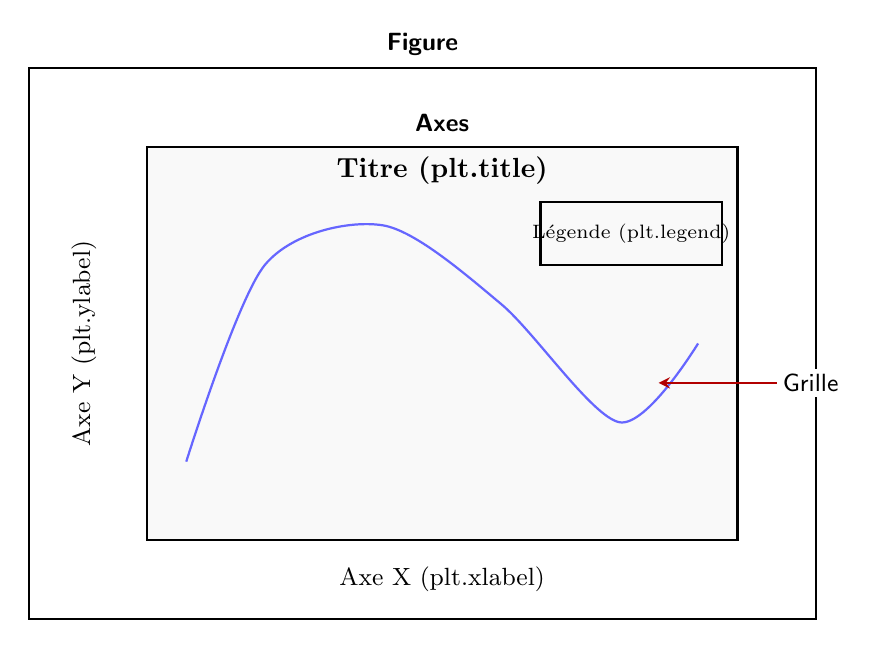
\begin{tikzpicture}[
    zone/.style={rectangle, draw, dashed, rounded corners},
    lbl/.style={font=\small\sffamily, fill=white, inner sep=2pt},
    arr/.style={->, thick, >=stealth, red!70!black}
]
% Figure frame
\draw[thick] (0,0) rectangle (10,7);
\node[lbl] at (5, 7.3) {\textbf{Figure}};

% Axes area
\draw[thick, fill=gray!5] (1.5, 1) rectangle (9, 6);
\node[lbl] at (5.25, 6.3) {\textbf{Axes}};

% Title
\node[font=\bfseries] at (5.25, 5.7) {Titre (\py{plt.title})};

% Fake curve
\draw[blue!60, thick, smooth] plot coordinates
    {(2,2) (3,4.5) (4.5,5) (6,4) (7.5,2.5) (8.5,3.5)};

% X label
\node[font=\small] at (5.25, 0.5) {Axe X (\py{plt.xlabel})};

% Y label
\node[font=\small, rotate=90] at (0.7, 3.5) {Axe Y (\py{plt.ylabel})};

% Legend box
\draw[thick] (6.5, 4.5) rectangle (8.8, 5.3);
\node[font=\scriptsize] at (7.65, 4.9) {L\'egende (\py{plt.legend})};

% Grid annotation
\draw[arr] (9.5, 3) -- (8, 3);
\node[lbl, right] at (9.5, 3) {Grille};
\end{tikzpicture}
\caption{Anatomie d'une figure Matplotlib~: figure, axes, titre, \'etiquettes et l\'egende.}
\label{fig:matplotlib-anatomie}
\end{figure}

% ============================================================
\section{Nuages de points~: \py{plt.scatter()}}
\index{plt.scatter}

\begin{codeblock}[title=\textbf{Python}]
\begin{minted}{python}
import numpy as np
import matplotlib.pyplot as plt

# Simuler des données expérimentales
rng = np.random.default_rng(42)
n = 50
concentration = rng.uniform(0, 10, n)
absorbance = 0.42 * concentration + rng.normal(0, 0.3, n)

plt.scatter(concentration, absorbance, color="blue", alpha=0.6,
            label="Mesures")

# Droite de régression
coeffs = np.polyfit(concentration, absorbance, 1)
x_fit = np.linspace(0, 10, 100)
plt.plot(x_fit, np.polyval(coeffs, x_fit), "r-",
         label=f"Régression : y = {coeffs[0]:.2f}x + {coeffs[1]:.2f}")

plt.xlabel("Concentration (mol/L)")
plt.ylabel("Absorbance")
plt.title("Loi de Beer-Lambert")
plt.legend()
plt.grid(True, alpha=0.3)
plt.show()
\end{minted}
\end{codeblock}

\begin{codeoutput}
\begin{verbatim}
[Figure affichée : nuage de points bleus avec droite de régression rouge,
titre « Loi de Beer-Lambert », axes étiquetés.]
\end{verbatim}
\end{codeoutput}

% ============================================================
\section{Histogrammes~: \py{plt.hist()}}
\index{plt.hist}

\begin{codeblock}[title=\textbf{Python}]
\begin{minted}{python}
import numpy as np
import matplotlib.pyplot as plt

rng = np.random.default_rng(42)

# Distribution des masses d'un échantillon
masses = rng.normal(loc=75, scale=8, size=1000)

plt.hist(masses, bins=30, color="green", alpha=0.7,
         edgecolor="black", density=True)
plt.xlabel("Masse (kg)")
plt.ylabel("Densité de probabilité")
plt.title("Distribution des masses (n = 1000)")
plt.axvline(np.mean(masses), color="red", linestyle="--",
            label=f"Moyenne = {np.mean(masses):.1f} kg")
plt.legend()
plt.show()
\end{minted}
\end{codeblock}

\begin{codeoutput}
\begin{verbatim}
[Figure affichée : histogramme vert avec 30 barres,
ligne rouge en pointillés marquant la moyenne.]
\end{verbatim}
\end{codeoutput}

% ============================================================
\section{Diagrammes en barres~: \py{plt.bar()}}
\index{plt.bar}

\begin{codeblock}[title=\textbf{Python}]
\begin{minted}{python}
import matplotlib.pyplot as plt

elements = ["H", "C", "N", "O", "S"]
abondance = [63.0, 9.5, 1.4, 25.5, 0.6]  # % dans le corps humain

plt.bar(elements, abondance, color=["red", "gray", "blue",
        "cyan", "yellow"], edgecolor="black")
plt.xlabel("Élément chimique")
plt.ylabel("Abondance (%)")
plt.title("Composition élémentaire du corps humain")
plt.show()
\end{minted}
\end{codeblock}

\begin{codeoutput}
\begin{verbatim}
[Figure affichée : diagramme en barres colorées montrant
l'abondance des éléments dans le corps humain.]
\end{verbatim}
\end{codeoutput}

% ============================================================
\section{Sous-graphiques~: \py{plt.subplots()}}
\index{subplots}

\begin{codeblock}[title=\textbf{Python}]
\begin{minted}{python}
import numpy as np
import matplotlib.pyplot as plt

x = np.linspace(0, 4 * np.pi, 300)

fig, axes = plt.subplots(2, 2, figsize=(10, 8))

# sin(x)
axes[0, 0].plot(x, np.sin(x), color="blue")
axes[0, 0].set_title("sin(x)")
axes[0, 0].grid(True)

# cos(x)
axes[0, 1].plot(x, np.cos(x), color="red")
axes[0, 1].set_title("cos(x)")
axes[0, 1].grid(True)

# exp(-x/5) * sin(x)  — signal amorti
axes[1, 0].plot(x, np.exp(-x / 5) * np.sin(x), color="green")
axes[1, 0].set_title("Signal amorti")
axes[1, 0].grid(True)

# x² et x³
axes[1, 1].plot(x, x**2, label="$x^2$")
axes[1, 1].plot(x, x**3 / 10, label="$x^3/10$")
axes[1, 1].set_title("Polynômes")
axes[1, 1].legend()
axes[1, 1].grid(True)

plt.tight_layout()
plt.show()
\end{minted}
\end{codeblock}

\begin{codeoutput}
\begin{verbatim}
[Figure affichée : grille 2×2 de sous-graphiques avec
sin(x), cos(x), signal amorti et polynômes.]
\end{verbatim}
\end{codeoutput}

\begin{bonnepratique}
Utilisez toujours \py{plt.tight\_layout()} ou \py{fig.tight\_layout()} pour \'eviter
que les \'etiquettes se chevauchent entre sous-graphiques.
\end{bonnepratique}

% ============================================================
\section{Personnalisation avanc\'ee}
\index{personnalisation}

\begin{codeblock}[title=\textbf{Python}]
\begin{minted}{python}
import numpy as np
import matplotlib.pyplot as plt

t = np.linspace(0, 10, 500)
y1 = np.sin(2 * np.pi * 0.5 * t)
y2 = np.sin(2 * np.pi * 1.0 * t)

plt.figure(figsize=(10, 5))
plt.plot(t, y1, "b-", linewidth=2, label="f = 0.5 Hz")
plt.plot(t, y2, "r--", linewidth=1.5, label="f = 1.0 Hz")

plt.xlabel("Temps (s)", fontsize=14)
plt.ylabel("Amplitude", fontsize=14)
plt.title("Signaux sinusoïdaux", fontsize=16, fontweight="bold")
plt.legend(fontsize=12, loc="upper right")
plt.xlim(0, 10)
plt.ylim(-1.5, 1.5)
plt.grid(True, alpha=0.3)

# Annotation
plt.annotate("Maximum", xy=(0.5, 1), xytext=(2, 1.3),
             arrowprops=dict(arrowstyle="->"), fontsize=11)

plt.show()
\end{minted}
\end{codeblock}

\begin{codeoutput}
\begin{verbatim}
[Figure affichée : deux signaux sinusoïdaux avec styles différents,
annotation fléchée pointant vers le maximum.]
\end{verbatim}
\end{codeoutput}

% ============================================================
\section{Sauvegarder une figure~: \py{plt.savefig()}}
\index{plt.savefig}

\begin{codeblock}[title=\textbf{Python}]
\begin{minted}{python}
import numpy as np
import matplotlib.pyplot as plt

x = np.linspace(-5, 5, 200)
y = np.exp(-x**2 / 2) / np.sqrt(2 * np.pi)

plt.plot(x, y, "k-", linewidth=2)
plt.fill_between(x, y, alpha=0.3)
plt.xlabel("x")
plt.ylabel("f(x)")
plt.title("Distribution normale standard")

# Sauvegarder en haute résolution
plt.savefig("gaussienne.png", dpi=300, bbox_inches="tight")
plt.savefig("gaussienne.pdf", bbox_inches="tight")
print("Figure sauvegardée en PNG et PDF.")
\end{minted}
\end{codeblock}

\begin{codeoutput}
\begin{verbatim}
Figure sauvegardée en PNG et PDF.
\end{verbatim}
\end{codeoutput}

\begin{attention}
Appelez \py{plt.savefig()} \textbf{avant} \py{plt.show()}, sinon la figure sera
vide lors de la sauvegarde. L'option \py{bbox\_inches="tight"} \'evite de couper
les \'etiquettes.
\end{attention}

% ============================================================
\section{Figures scientifiques~: trajectoire d'un projectile}

\begin{codeblock}[title=\textbf{Python}]
\begin{minted}{python}
import numpy as np
import matplotlib.pyplot as plt

g = 9.81
angles = [30, 45, 60, 75]  # degrés
v0 = 20  # m/s

plt.figure(figsize=(10, 6))

for theta_deg in angles:
    theta = np.radians(theta_deg)
    t_vol = 2 * v0 * np.sin(theta) / g
    t = np.linspace(0, t_vol, 200)
    x = v0 * np.cos(theta) * t
    y = v0 * np.sin(theta) * t - 0.5 * g * t**2
    plt.plot(x, y, linewidth=2, label=f"θ = {theta_deg}°")

plt.xlabel("Distance horizontale (m)", fontsize=13)
plt.ylabel("Hauteur (m)", fontsize=13)
plt.title("Trajectoire d'un projectile (v₀ = 20 m/s)", fontsize=14)
plt.legend(fontsize=11)
plt.grid(True, alpha=0.3)
plt.ylim(bottom=0)
plt.show()
\end{minted}
\end{codeblock}

\begin{codeoutput}
\begin{verbatim}
[Figure affichée : quatre trajectoires paraboliques pour différents
angles de lancement, montrant que 45° donne la portée maximale.]
\end{verbatim}
\end{codeoutput}

% ============================================================
\section{Erreurs courantes}

\begin{errmark}
\begin{enumerate}
    \item \textbf{Oublier \py{plt.show()}}~: dans un script (hors Jupyter), sans
    \py{plt.show()}, aucune fen\^etre ne s'affiche. La figure est cr\'e\'ee en m\'emoire
    mais reste invisible.

    \item \textbf{Mauvaise taille de figure}~: par d\'efaut, les figures sont petites.
    Utilisez \py{plt.figure(figsize=(largeur, hauteur))} pour contr\^oler la taille
    en pouces.

    \item \textbf{Sauvegarder apr\`es \py{plt.show()}}~: \py{plt.show()} vide la figure
    en cours. Tout appel \`a \py{plt.savefig()} apr\`es donnera un fichier vide.

    \item \textbf{Confondre \py{plt.plot} et l'interface orient\'ee objet}~: pour des
    sous-graphiques, utilisez \py{ax.plot()} et non \py{plt.plot()} qui agit sur
    le dernier axe actif.

    \item \textbf{Oublier les \'etiquettes}~: un graphique sans titre ni \'etiquettes
    d'axes est inutilisable en contexte scientifique. Ajoutez \emph{toujours}
    \py{xlabel}, \py{ylabel} et \py{title}.
\end{enumerate}
\end{errmark}

% ============================================================
\section{Mini-projet~: Visualisation du mouvement d'un projectile}

\begin{projet}
Cr\'eez un programme complet qui~:
\begin{enumerate}
    \item Demande la vitesse initiale $v_0$ et l'angle de lancement $\theta$.
    \item Calcule la trajectoire, la port\'ee et la hauteur maximale.
    \item Produit une figure avec~:
    \begin{itemize}
        \item La trajectoire parabolique.
        \item Un point marqu\'e au sommet (hauteur max).
        \item Une annotation indiquant la port\'ee.
        \item Un encadr\'e avec les param\`etres ($v_0$, $\theta$, port\'ee, $h_{\max}$).
    \end{itemize}
    \item Sauvegarde la figure en PDF.
\end{enumerate}
\end{projet}

\begin{codeblock}[title=\textbf{Python}]
\begin{minted}{python}
import numpy as np
import matplotlib.pyplot as plt

v0 = 25.0       # m/s
theta_deg = 55   # degrés
g = 9.81

theta = np.radians(theta_deg)
t_vol = 2 * v0 * np.sin(theta) / g
portee = v0**2 * np.sin(2 * theta) / g
h_max = (v0 * np.sin(theta))**2 / (2 * g)
t_max = v0 * np.sin(theta) / g

t = np.linspace(0, t_vol, 300)
x = v0 * np.cos(theta) * t
y = v0 * np.sin(theta) * t - 0.5 * g * t**2

fig, ax = plt.subplots(figsize=(10, 6))
ax.plot(x, y, "b-", linewidth=2.5)
ax.plot(v0 * np.cos(theta) * t_max, h_max, "ro", markersize=10)
ax.annotate(f"Sommet\n({h_max:.1f} m)",
            xy=(v0 * np.cos(theta) * t_max, h_max),
            xytext=(portee * 0.6, h_max * 0.95),
            arrowprops=dict(arrowstyle="->"), fontsize=11)

info = (f"v₀ = {v0} m/s\n"
        f"θ = {theta_deg}°\n"
        f"Portée = {portee:.1f} m\n"
        f"h_max = {h_max:.1f} m")
ax.text(0.02, 0.95, info, transform=ax.transAxes,
        fontsize=11, verticalalignment="top",
        bbox=dict(boxstyle="round", facecolor="wheat", alpha=0.8))

ax.set_xlabel("Distance (m)", fontsize=13)
ax.set_ylabel("Hauteur (m)", fontsize=13)
ax.set_title("Trajectoire d'un projectile", fontsize=15)
ax.set_ylim(bottom=0)
ax.grid(True, alpha=0.3)
plt.tight_layout()
plt.savefig("projectile.pdf", bbox_inches="tight")
plt.show()
print(f"Portée : {portee:.1f} m, Hauteur max : {h_max:.1f} m")
\end{minted}
\end{codeblock}

\begin{codeoutput}
\begin{verbatim}
Portée : 59.2 m, Hauteur max : 21.4 m
\end{verbatim}
\end{codeoutput}

% ============================================================
\section{Exercices}

\begin{exercice}[$\star$ --- Courbe exponentielle]
Tracez la fonction $f(x) = e^{-x/3} \cos(2\pi x)$ sur $[0, 10]$.
Ajoutez un titre, des \'etiquettes d'axes et une grille.
\end{exercice}

\begin{exercice}[$\star$ --- Histogramme de lancers de d\'es]
Simulez 10\,000 lancers de deux d\'es. Tracez l'histogramme de la somme obtenue.
Quelle somme est la plus fr\'equente~?
\end{exercice}

\begin{exercice}[$\star\star$ --- Diagramme de phases]
Tracez un diagramme de phases simplifi\'e de l'eau~: pression ($y$) en fonction de
la temp\'erature ($x$). Utilisez \py{plt.fill\_between} pour colorier les zones
solide, liquide et gazeuse.
\end{exercice}

\begin{exercice}[$\star\star$ --- Sous-graphiques multiples]
Cr\'eez une figure $2\times 2$ montrant~: (a) $\sin(x)$, (b) $\cos(x)$,
(c) $\tan(x)$ (limit\'e \`a $[-5, 5]$), (d) $e^x$ et $\ln(x)$.
Chaque sous-graphique doit avoir son titre et sa grille.
\end{exercice}

\begin{exercice}[$\star\star\star$ --- Carte de chaleur]
Cr\'eez une matrice $20\times 20$ repr\'esentant la temp\'erature d'une plaque
chauffante (bords froids \`a 0\,\textdegree C, centre chaud \`a 100\,\textdegree C).
Affichez-la avec \py{plt.imshow()} et ajoutez une barre de couleur.
\emph{Indice}~: initialisez une matrice de z\'eros et ajoutez une gaussienne
centr\'ee.
\end{exercice}

% ============================================================
\begin{formules}{R\'esum\'e du chapitre~: Matplotlib}
\begin{itemize}
    \item \textbf{Courbes}~: \py{plt.plot(x, y, style, label=...)}
    \item \textbf{Nuages}~: \py{plt.scatter(x, y, color=..., alpha=...)}
    \item \textbf{Histogrammes}~: \py{plt.hist(data, bins=..., density=True)}
    \item \textbf{Barres}~: \py{plt.bar(categories, valeurs)}
    \item \textbf{Sous-graphiques}~: \py{fig, axes = plt.subplots(nrows, ncols)}
    \item \textbf{\'Etiquettes}~: \py{plt.xlabel}, \py{plt.ylabel}, \py{plt.title}
    \item \textbf{L\'egende}~: \py{plt.legend()} (apr\`es avoir utilis\'e \py{label=...})
    \item \textbf{Grille}~: \py{plt.grid(True)}
    \item \textbf{Sauvegarde}~: \py{plt.savefig("nom.pdf", dpi=300, bbox\_inches="tight")}
    \item \textbf{R\`egle d'or}~: \py{savefig} \emph{avant} \py{show}
\end{itemize}
\end{formules}
